%% ------------------------------------------------------------------------- %%n
\chapter{Experimentos e Resultados Preliminares}
\label{cap:Experimentos_Resultados}


Nesse capítulo serão apresentados alguns experimentos preliminares que foram feitos com dados sintéticos e com reais de Plâncton. 

\section{Framework de Aprendizado Ativo Utilizado}
\label{sec:framework_al}

O framework utilizado nesses experimentos foram baseados no trabalho de [\cite{saito2014active}]. A figura ~\ref{fig:priscila_algoritmo} e os seguintes passos explicam as etapas:

\begin{figure}
  \centering
  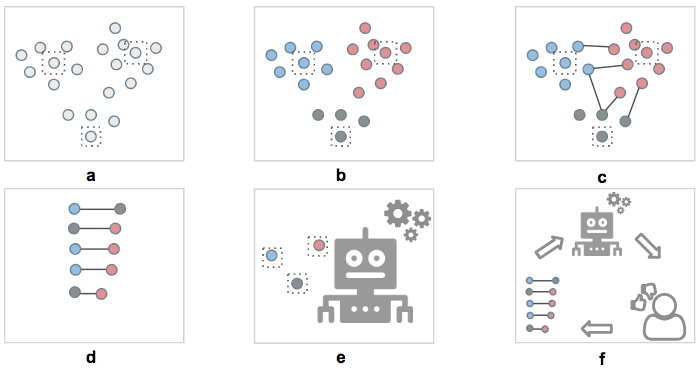
\includegraphics[width=0.8\textwidth]{figures/priscila_algoritmo.png}
  \caption{Framework Utilizado nos Experimentos}
  \label{fig:priscila_algoritmo}
\end{figure}




\begin{enumerate}
  \item No primeiro quadro (a), temos um conjunto de dados que representam um espaço de features. Inicialmente esses dados não estão rotulados, então não sabemos quais suas verdadeiras classes. Temos a informação de quantas classes podem existir para esses dados;
  \item Em (b), aplicamos um algoritmo não-supervisionado de clusterização. No nosso caso utilizamos o K-means e utilizamos como k duas vezes o número de classes possíveis;
  \item No (c), a partir do momento que temos os K-clusters, aplicamos o algoritmo de vizinhos próximos KNN para gerarmos um grafo. O número de vizinhos foi escolhido de forma prática;
  \item Em (d), reduzimos o dataset original para os dados que possuem alguma relação KNN com vizinhos que sejam diferentes da classe do seu respectivo cluster. A ideia é que tenhamos apenas os dados que estejam na borda dos cluters pois eles são mais representativos;
  \item Ainda em (d), ordenamos as amostras do dataset reduzido, de maneira decrescente, através da distância euclidiana das arestas. Iniciamos por elas pois temos como premisa que uma maior distância pode representar amostras mais relevantes;
  \item Nos quadros (e) e (f), como sabemos os rótulos verdadeiros dos dados, geramos um classificador através dos centroides dos clusters. Esses dados compõe um novo dataset que será utilizado como base de treinamento. A partir disso entramos no ciclo do Aprendizado Ativo. A cada inicio do ciclo, selecionamos n amostras do dataset reduzido e o classificador gera as previsões dos dados. Comparamos o resultado com os rótulos verdadeiros e, caso esteja incorreto, corrigimos e incorporamos esse dados para a base de treinamento. Esse ciclo continua até que os dados disponíveis no dataset reduzido acabem. 
\end{enumerate}

No caso dos dados rândomicos seguimos a mesma lógica até o passo 2. A partir disso geramos um classificador também pelos centróids a iniciamos um ciclo de aprendizado onde, a cada ciclo, selecionamos n dados, com a diferença de ser de forma rândomica.

\section{Experimentos com Dados Sintéticos}
\label{sec:experimentos_sinteticos}

Para os experimentos com dados sintéticos, geramos um dataset com 1000 amostras que representam um espaço de features 2D. A figura ~\ref{fig:exemplo_sintetico_1} mostra do lado esquerdo os dados gerados sem nenhuma classe, enquanto o lado direito mostra os rótulos verdadeiros. 


\begin{figure}
  \centering
  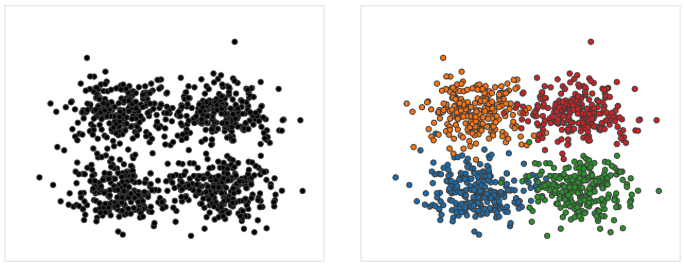
\includegraphics[width=0.9\textwidth]{figures/toy_example_1.png}
  \caption{Exemplo Sintético}
  \label{fig:exemplo_sintetico_1}
\end{figure}

Aplicamos o framework anterior neste dataset. Como temos como premissa que são quatro classes possíveis, utilizamos no K-means oito clusters. A partir disso aplicamos o algoritmo de KNN e obtemos a relações de interesse, conforme a figura ~\ref{fig:exemplo_sintetico_2}. 

\begin{figure}
  \centering
  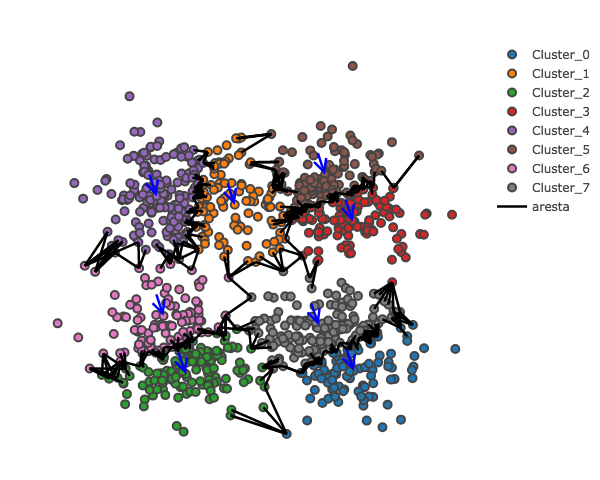
\includegraphics[width=0.8\textwidth]{figures/toy_example_2.png}
  \caption{Exemplo Sintético}
  \label{fig:exemplo_sintetico_2}
\end{figure}

É interessante notar que algumas amostras podem não ser tão relevantes pois pertencem ao mesmo grupo. Por exemplo os clusters laranja (1) e roxo (4), na imagem ~\ref{fig:exemplo_sintetico_2}, que pertencem à mesma classe. Apesar disso, como o classificador será treinado inicialmente com o centroide de cada classe, é provável que a predição convirja rapidamente. De qualquer forma, os dados mais relevantes estão entre as amostras que não são da mesma classe. 


\begin{figure}
  \centering
  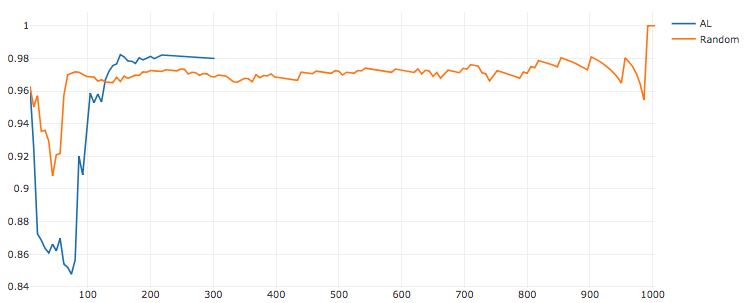
\includegraphics[width=0.9\textwidth]{figures/grafico_exemplo_sintetico.png}
  \caption{Gráfico com Resultados dos Dados Sintéticos}
  \label{fig:grafico_exemplo_sintetico}
\end{figure}

Fizemos os testes com a abordagem do Aprendizado Ativo e através de forma randômica. Escolhemos dez vizinhos próximos para encontrar as arestas e isso nos gerou um total de 300 dados, o que representa um redução de 70\% do dataset original. O gráfico ~\ref{fig:grafico_exemplo_sintetico} mostra a performance de ambos frameworks. É interessante notar que inicialmente o framework de Aprendizado Ativo não possui uma boa acurácia mas, após algumas amostras, entra numa sequência crescente, chegando em 98\% com 302 amostras, enquanto, se selecionamos os dados de forma randômica chegamos em 96.88\%. Além disso, com os dados aleatórios, atingimos um valor de 98\% apenas a partir das 900 amostras. Apesar de ambos os resultados terem uma boa taxa de acerto (provavelmente por ser um exemplo simples), o framework de Aprendizado Ativo mostrou a mesma taxa de acerto que a forma randômica com 1/3 de amostras necessárias. 


\section{Experimentos com Dados de Plâncton}
\label{sec:experimentos_plancton}

Para os experimentos com dados de Plâncton utilizamos a base de dados da FURG e escolhemos apenas 6 classes possíveis de Plâncton. A figura ~\ref{fig:Plancton_Exemplos} mostra alguns exemplos de imagens.Quando aplicado o K-means foi utilizado doze clusters, seguindo a mesma lógica de termos o dobro de clusters para o máximo esperado de classes. Para os vizinhos próximos foi utilizado o valor de 8 vizinhos. 

\begin{figure}
  \centering
  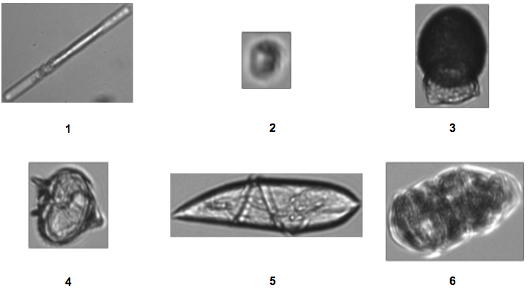
\includegraphics[width=0.6\textwidth]{figures/Plancton_Exemplos.png}
  \caption{Exemplos de Imagens de Plâncton Utilizadas. As classes são 1:Bacillariophycidae-1, 2:Prorocentrales, 3:Spirotrichea, 4:Peridiniales, 5:Gymnodiniales, 6:Cochlodinium}
  \label{fig:Plancton_Exemplos}
\end{figure}


\begin{figure}
  \centering
  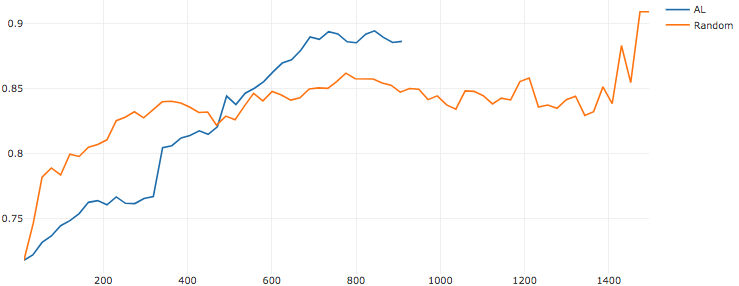
\includegraphics[width=0.9\textwidth]{figures/grafico_exemplo_plancton.png}
  \caption{Gráfico com Resultados dos Dados de Plâncton}
  \label{fig:grafico_exemplo_plancton}
\end{figure}

Assim como ocorreu com os exemplo sintético, os resultados mostraram que, nas primeiras interações, o framework de Aprendizado Ativo é inferior ao randômico mas, a partir da interação 22, com 471 dados, os dois frameworks possuem a mesma acurácia de 82\%. Desta interação em diante o Aprendizado Ativo apenas melhora sua performance, enquando os dados aleatórios permanecem em uma tendência constante. No final, com cerca de 900 amostras, o framework de Aprendizado Ativo chega em uma acurácia de 88.62\%. Os dados aleatórios só chegam nessa acurácia com cderca de 1400 amostras. Isto é, com 2/3 do esforço atingimos a mesma acurácia.